\section{\texorpdfstring{$\mathcal{O}$}{O}-Notation}

\toclesssubsection{Motivation / Definition}

\begin{frame}{$\mathcal{O}$-Notation}{Motivation}
  \textbf{We are interested in:}
  \begin{itemize}
    \item
      Growth of a function in runtime $T(n)$
    \begin{itemize}
      \item
        Runtime of \textit{Minsort} qubic with $n^2$
      \item
         Runtime of \textit{HeapSort} nearly linear with $n \, \log n$
    \end{itemize}
    \item
      Describe the growth of the function
    \begin{itemize}
      \item
        We use
        {\color{Mittel-Blau}$\mathcal{O}(n)$},
        {\color{Mittel-Blau}$\Omega (n)$},
        {\color{Mittel-Blau}$\Theta (n)$}
        (Big O / Omega / Theta of $n$)\\
        (Landau-Symbols \cite{wikipedia_big_o_notation})
    \end{itemize}
  \end{itemize}
\end{frame}

%-------------------------------------------------------------------------------

\begin{frame}{$\mathcal{O}$-Notation}{Definition}
  \textbf{Big $\mathcal{O}$-Notation:}
  \begin{itemize}
    \item
      We look at the function:
      $f\!: \mathbb{N} \to \mathbb{R}, \; n \mapsto f(n)$
      \begin{itemize}
        \item
          $\mathbb{N}\!:$ Natural numbers $\rightarrow$ input size
        \item
          $\mathbb{R}\!:$ Real numbers $\rightarrow$ runtime
      \end{itemize}
   \item
     \textbf{Example:}
   \begin{itemize}
     \item
       $f(n) = 3 \, n$
     \item
       $f(n) = 2 \, n \, \log n$
     \item
       $f(n) = \frac{1}{10} n^2$
     \item
       $f(n) = n^2 + 3 \, n \, \log n - 4 \, n$
    \end{itemize}
  \end{itemize}
\end{frame}

%-------------------------------------------------------------------------------

\begin{frame}{$\mathcal{O}$-Notation}{Definition}
  \textbf{Big $\mathcal{O}$-Notation:}
  \begin{itemize}
    \item
      $f,g\!: \mathbb{N} \to \mathbb{R}$
    \item
      \textbf{Intuitive:}\\
      $f$ is $\mathcal{O}(g)$ if $f$ relative to $g$ does not grow faster than 
      $g$
    \item 
      \textbf{Informal:}\\ 
      $f \in \mathcal O(g)$: From a value $n_0$ for all
      $n \geq n_0 \rightarrow f(n) \leq C \cdot g(n)$
  \end{itemize}
  \begin{block}{\textbf{Formal:} $f \in \mathcal O(g)$}
    \begin{math}
      \mathcal O(g) = \lbrace f: \mathbb{N} \to \mathbb{R} ~ | ~
        \exists n_0 \in \mathbb{N}, \, \forall n > n_0, \, \exists C > 0: \,
        f(n) \leq C \cdot g(n)\rbrace
    \end{math}
  \end{block}
\end{frame}

%-------------------------------------------------------------------------------

\subsection{Examples}

\begin{frame}{$\mathcal{O}$-Notation}{Examples}
  \textbf{Illustration of the Big O-Notation:}\\[-1.0em]
  \begin{columns}
    \begin{column}{0.9\textwidth}
      \begin{figure}[!h]
        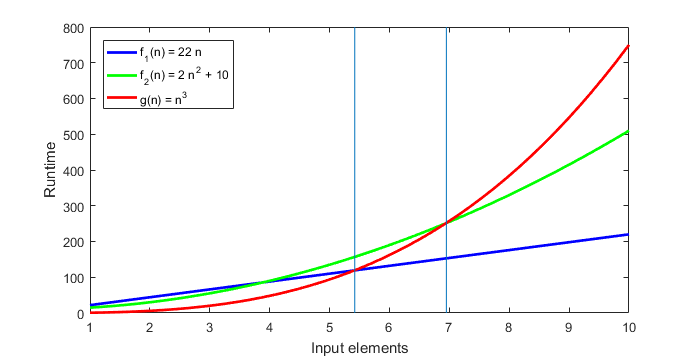
\includegraphics[width=\linewidth]{Images/BigONotationRuntime.png}
        \caption{Runtime of two algorithms $f_1, f_2$}
        \label{fig:big_o_runtime_example}
      \end{figure}
    \end{column}
    \begin{column}{0.1\textwidth}
      \vspace{-4.75em}\\
      \hspace*{-2.5em}$g(n)$\\[2.0em]
      \hspace*{-2.5em}$f_2 \in \mathcal{O}(g)$\\[2.5em]
      \hspace*{-2.5em}$f_1 \in \mathcal{O}(g)$
    \end{column}
  \end{columns}
\end{frame}

%-------------------------------------------------------------------------------

\begin{frame}{$\mathcal{O}$-Notation}{Examples}
  \textbf{Example:}
  \begin{itemize}
    \item
      $f(n) = 5 \, n + 7, \; g(n) = n$\\
      $\Rightarrow$ $5 \, n + 7 \in \mathcal{O}(g)$\\
      $\Rightarrow f \in \mathcal{O}(g)$
     \item
      \textbf{Intuitive:}\\
      $f(n) = 5 \, n + 7$ $\rightarrow$ linear
  \end{itemize}
  \begin{alertblock}{Attention}
    $f(n) \leq g(n)$ is not correct, better is
    $f(n) \leq C \cdot g(n) \;\; \forall n > n_0$.
  \end{alertblock}
\end{frame}

%-------------------------------------------------------------------------------

\begin{frame}{$\mathcal{O}$-Notation}{Proof}
  \begin{proof}[
    We have to proof:
    \begin{math}
      \exists n_0, \, \exists C, \, \forall n \geq n_0 \! : \;
        5 \, n + 7 \leq C \cdot n
    \end{math}
  ]
    \begin{eqnarray*}
      &5 \, n + 7 &\leq \;\; 5 \, n + n \hspace{1em} (\text{for} ~ n \geq 7)\\
      && \leq \;\; 6 \, n
    \end{eqnarray*}
    $\hspace{1.5em} \Rightarrow n_0 = 7, \, C = 7$ \qedhere
  \end{proof}
\end{frame}

%-------------------------------------------------------------------------------

\begin{frame}{$\mathcal{O}$-Notation}{Proof}
  \begin{proof}[Alternate proof:]
    \begin{eqnarray*}
      &5 \, n + 7 &\leq \;\; 5 \, n + 7 \, n \hspace{1em}
      (\text{for} ~ n \geq 1)\\
      && \leq \;\; 12 \, n
    \end{eqnarray*}
    $\hspace{1.5em} \Rightarrow n_0 = 1, \, C = 12$ \qedhere
  \end{proof}
\end{frame}

%-------------------------------------------------------------------------------

\begin{frame}{$\mathcal{O}$-Notation}{Examples}
  \textbf{Big O-Notation:}
  \begin{itemize}
    \item
      We are only interested in the terms which are growing the fastest,
      the others will be ignored
    \item
      $f(n)$ is limited {\color{Mittel-Blau}from above} by $c \cdot g(n)$
  \end{itemize}
  \textbf{Examples:}
  \begin{align*}
     2 \, n^2 + 7 \, n - 20 \in & \,\mathcal{O}(n^2)\\
     2 \, n^2 + 7 \, n \, \log n - 20 \in & {}\\
     7 \, n \, \log n - 20 \in & {}\\
     5 \in & {}\\
     2 \, n^2 + 7 \, n \, \log n + n^3 \in & {}\\
     2 \sqrt{x} + 3 \ln x \in & \mathcal{O}(?)
  \end{align*}
\end{frame}

%-------------------------------------------------------------------------------

\section{\texorpdfstring{$\Omega$}{Omega}-Notation}

\begin{frame}{$\Omega$-Notation}{Definition}
  \textbf{Omega-Notation:}
  \begin{itemize}
    \item
      \textbf{Intuitive}:\\
      $f \in \Omega(g)$, $f$ is growing at least as fast as $g$
  \end{itemize}
 	\begin{block}{\textbf{Formal:} $f \in \Omega(g)$}
    \begin{math}
      \Omega(g) = \lbrace f: \mathbb{N} \to \mathbb{R} ~ | ~
        \exists n_0 \in \mathbb{N}, \, \forall n > n_0, \, \exists C > 0: \,
        f(n) \geq C \cdot g(n)\rbrace
    \end{math}
 	\end{block}
\end{frame}

%-------------------------------------------------------------------------------

\begin{frame}{$\Omega$-Notation}{Proof}
  \begin{proof}[Proof of $f(n) \in \Omega(g)$:]
    \begin{eqnarray*}
      &\underbrace{5 \, n + 7}_{f(n)} &\geq \;\; \underbrace{n}_{g(n)} 
      \hspace{1em} (\text{for} ~ n \geq 1)
    \end{eqnarray*}
    $\hspace{1.5em} \Rightarrow n_0 = 1, \, C = 1$ \qedhere
  \end{proof}
\end{frame}

%-------------------------------------------------------------------------------

\begin{frame}{$\Omega$-Notation}{Examples}
  \textbf{Illustration of the Omega-Notation:}\\[-1.0em]
  \begin{columns}
    \begin{column}{0.9\textwidth}
      \begin{figure}[!h]
        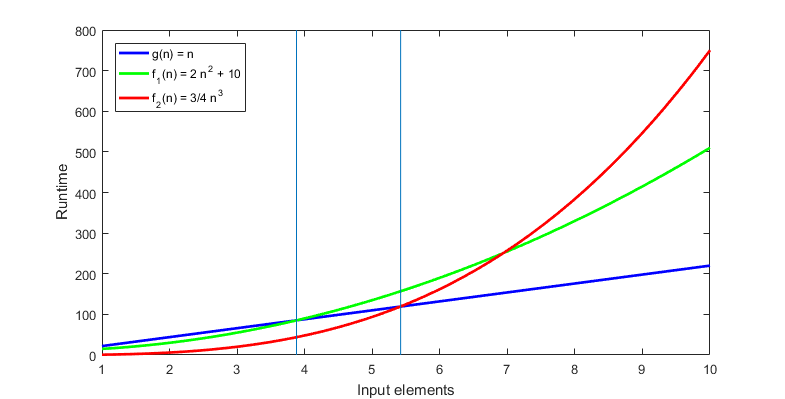
\includegraphics[width=\linewidth]{Images/OmegaNotationRuntime.png}
        \caption{Runtime of two algorithms $f_1, f_2$}
        \label{fig:omega_o_runtime_example}
      \end{figure}
    \end{column}
    \begin{column}{0.1\textwidth}
      \vspace{-4.75em}\\
      \hspace*{-2.5em}$f_2 \in \Omega(g)$\\[2.0em]
      \hspace*{-2.5em}$f_1 \in \Omega(g)$\\[2.5em]
      \hspace*{-2.5em}$g(n)$
    \end{column}
  \end{columns}
\end{frame}

%-------------------------------------------------------------------------------

\begin{frame}{$\Omega$-Notation}{Examples}
  \textbf{Big Omega-Notation:}
  \begin{itemize}
    \item
      We are only interested in the terms which are growing the fastest, the
      others will be ignored
    \item
      $f(n)$ is limited {\color{Mittel-Blau}from underneath} by
      $c \cdot g(n)$.\\
  \end{itemize}
  \textbf{Examples:}
  \begin{align*}
    2 \, n^2 + 7 \, n - 20 \in & \,\Omega(n^2)\\
    2 \, n^2 + 7 \, n \, \log n - 20 \in & {}\\
    7 \, n \, \log n - 20 \in & {}\\
    5 \in & {}\\
    2 \, n^2 + 7 \, n \, \log n + n^3 \in & {}
  \end{align*}
\end{frame}

%-------------------------------------------------------------------------------

\section{\texorpdfstring{$\Theta$}{Theta}-Notation}

\begin{frame}{$\Theta$-Notation}{Definition}
  \textbf{Theta-Notation:}
  \begin{itemize}
    \item
      \textbf{Intuitive}:\\
      $f \in \Theta(g)$, $f$ is growing at the same speed as $g$
  \end{itemize}
 	\begin{block}{\textbf{Formal:} $f \in \Theta(g)$}
 		$\Theta(g) = \underbrace{\mathcal O(g) \cap \Omega(g)}_{Intersection}$
 	\end{block}
  \textbf{Example:}\\
  \hspace*{1.5em}$f(n) = 5 \, n + 7, \;
    f(n) \in \mathcal{O}(n), \,
    f(n) \in \Omega(n)$\\
  \hspace*{3.0em}$\Rightarrow f(n) \in \Theta(n)$\\[0.5em]
  \begin{center}
   \textit{Proof for $\mathcal{O}(g)$ and $\Omega(g)$ look at slides 12 and 15}
  \end{center}
\end{frame}

%-------------------------------------------------------------------------------

\section{Runtime}

\toclesssubsection{Summary}

\begin{frame}{Runtime}{Landau-Symbol Summary}
  \textbf{Big O-Notation} $\mathcal{O}(n)$\textbf{:}\\
    \begin{itemize}
      \item
        $f$ is growing {\color{Mittel-Blau}at least} as fast as $g$
      \item
        $C \cdot g(n)$ is the upper bound
    \end{itemize}
  \textbf{Big Omega-Notation} $\Omega(n)$\textbf{:}\\
  \begin{itemize}
    \item
      $f$ is growing {\color{Mittel-Blau}at maximum} as fast as $g$
    \item
      $C \cdot g(n)$ is the lower bound
  \end{itemize}
  \textbf{Big Theta-Notation} $\Theta(n)$\textbf{:}\\
  \begin{itemize}
    \item
      $f$ is growing at {\color{Mittel-Blau}the same} speed as $g$
      \begin{itemize}
        \item
          $C_1 \cdot g(n)$ is the lower bound
        \item
          $C_2 \cdot g(n)$ is the upper bound
      \end{itemize}
  \end{itemize}
\end{frame}

%-------------------------------------------------------------------------------

\begin{frame}{Runtime}{Common Runtimes}
  \begin{table}[!h]
    \begin{center}
      \caption{Common runtime types}
      \label{RuntimeTable}
      \begin{tabularx}{\textwidth}{XX}
        Runtime & Growth\\
        \hline
        $f \in \Theta (1)$ & constant time\\
        $f \in \Theta (\log n) = \Theta (\log_k n)$ & logarithmic time\\
        $f \in \Theta (n)$ & linear time\\
        $f \in \Theta (n \, \log n)$ & n-log-n time (nearly linear)\\
        \hline
        $f \in \Theta (n^2)$ & squared time\\
        $f \in \Theta (n^3)$ & cubic time\\
        $f \in \Theta (n^k)$ & polynomial time\\
        \hline
        $f \in \Theta (k^n)$, $f \in \Theta(2^n)$ & exponential time
      \end{tabularx}
    \end{center}
  \end{table}
\end{frame}

%-------------------------------------------------------------------------------

\subsection{Limit / Convergence}

\begin{frame}{$\mathcal{O}$-Notation}{Limit / Convergence}
  \textbf{Definition of \enquote{Limit}}
  \begin{itemize}
    \item
      The limit of an indefinite progression $f$ is $L$
    \item
      A function $f\!: \mathbb{N} \rightarrow \mathbb{R}$ can be written as a
      progression\\
      $\Rightarrow$ $\lim\limits_{n \rightarrow \infty}$ $f_n$ = $L$
  \end{itemize}
  \begin{block}{Convergence}
    \begin{math}
      \forall \epsilon > 0 \; \exists n_0 \in \mathbb{N} \;\;
      \forall n \geq n_0 \! : \; \Vert f_n - L \Vert \leq \epsilon
    \end{math}
  \end{block}
\end{frame}

%-------------------------------------------------------------------------------

\begin{frame}{$\mathcal{O}$-Notation}{Limit / Convergence}
  \begin{proof}[Proof for $f(n) = 2 + \frac{1}{n}$:]
    $f\!: \mathbb{N} \to \mathbb{R}, \; n \mapsto 2 + \frac{1}{n}$
    \begin{eqnarray*}
      \lim_{n \to \infty} f(n)
        = \lim_{n \to \infty} 2 + \dfrac{1}{n}
        = 2
      & \Rightarrow \left\Vert 2 + \dfrac{1}{n} - 2 \right\Vert \leq \epsilon\\
      \Rightarrow n_0 = \left\lceil \dfrac{1}{\epsilon} \right\rceil
      \; \Rightarrow \; n \geq n_0
    \end{eqnarray*}
    \begin{eqnarray*}
      \left\lceil
        \frac{1}{n} \vphantom{\dfrac{1}{\frac{1}{\epsilon}}}
      \right\rceil
        = \dfrac{1}{n}
      \; \leq \;
      \dfrac{1}{n_0} = \left\lceil \dfrac{1}{\frac{1}{\epsilon}} \right\rceil
        = \epsilon
      \qedhere
    \end{eqnarray*}
  \end{proof}
\end{frame}

%-------------------------------------------------------------------------------

\begin{frame}{$\mathcal{O}$-Notation}{Limit / Convergence}
  Let $f,g \! : \; \mathbb{N} \to \mathbb{R}$ with an existing limit
  \[\lim_{n \to \infty} \dfrac{f(n)}{g(n)} = L\]
  So we can say:
  \begin{align}
    & f \in \mathcal{O}(g) & \Leftrightarrow
    && \lim_{n \to \infty} \dfrac{f(n)}{g(n)} < \infty\\
    & f \in \Omega(g) & \Leftrightarrow
    && \lim_{n \to \infty} \dfrac{f(n)}{g(n)} > 0\\
    & f \in \Theta(g) & \Leftrightarrow
    && 0 < \lim_{n \to \infty} \dfrac{f(n)}{g(n)} < \infty
  \end{align}
\end{frame}

%-------------------------------------------------------------------------------

\begin{frame}{$\mathcal{O}$-Notation}{Limit / Convergence}
  \[
    f \in \mathcal{O}(g)
    \; \Leftrightarrow \;
    \lim\limits_{n \rightarrow \infty} \frac{f(n)}{g(n)} < \infty
  \]
  \begin{proof}[Forward proof:]
     $f \in \mathcal{O}(g) \stackrel{\text{def. of }\mathcal{O}(n)}{\Rightarrow}
     \exists n_0, \, \forall n \geq n_0, \, \exists C\!:
     \; f(n) \leq C \cdot g(n)$
     \begin{alignat*}{2}
       {} && f(n) &\leq \; C \cdot g(n)\\
       \Rightarrow && \dfrac{f(n)}{g(n)} &\leq \; C\\
       \Rightarrow && \displaystyle
       \lim_{n \to \infty}\dfrac{f(n)}{g(n)} &\leq \; C
       \qedhere
      \end{alignat*}
  \end{proof}
\end{frame}

%-------------------------------------------------------------------------------

\begin{frame}{$\mathcal{O}$-Notation}{Limit / Convergence}
  \begin{proof}[Backward proof:]
    \begin{center}
      \vspace{-0.5em}
      \begin{math}
        \begin{aligned}
          & {} & \lim_{n \to \infty} \frac{f(n)}{g(n)} &< \; \infty\\
          & \Rightarrow & \lim_{n \to \infty} \frac{f(n)}{g(n)} &= \; L &&
          \hspace*{1.5em}\text{For some } L \in \mathbb{R} \text{ (Limit)}
        \end{aligned}
      \end{math}
      \vspace{1.0em}\\
      \begin{math}
        \begin{aligned}
          \stackrel{\text{def. limes}}{\Rightarrow} \hspace*{0.5em} &&
          \exists n_0, \, \forall n \geq n_0, \, \exists C\!: \hspace*{1.0em}&&
          \frac{f(n)}{g(n)} &\leq \; L + \varepsilon\\
          \Rightarrow \; &&
          \exists n_0, \, \forall n \geq n_0, \, \exists C\!: \hspace*{1.0em}&&
          f(n) &\leq \; \underbrace{(L + \varepsilon)}_{C} \cdot g(n)\\
          \Rightarrow \; &&
          f(n) \in \mathcal{O}(g)
          \qedhere
        \end{aligned}
      \end{math}
    \end{center}
  \end{proof}
\end{frame}